\subsection{RQ5: Predecessor language of interest of the respondents of new languages}
\label{RQ4}
We have confined our search into the predecessor language of interest of the \emph{expert developers}. According to our definition,  \emph{expert developers} are those developers who have answered at least one accepted answer.
To find the predecessor language of interest of the expert developers, we collected all the tags of the questions answered by expert developers and then sorted the tags according to their frequency to get the most frequent tags. The most frequent ten tags for each language is presented in Figure~\ref{fig:dev skills}.
% \begin{table}
\begin{center}
\begin{tabular}{|l|l|}
    \hline
    Developers & Tags in order of occurrence\\ \hline
    
    \multirow{2}{*}{Swift Developers}
    &iOS\\&Java\\&Objective-C\\&Swift\\&JavaScript\\&Android\\&iPhone\\&Php\\&C++\\&C\# \\ \hline
    
    \multirow{2}{*}{Go Developers}
    &Java  \\ &JavaScript\\ &Python \\&C++\\&Php\\&C\#\\&MySQL\\&C\\&Regex\\&JQuery \\ \hline
    
    \multirow{2}{*}{Rust Developers}
    &C++\\&C\\&Java\\&Python \\& Rust\\ &Ruby\\ &C\# \\ &Haskell \\ &JavaScript 	\\ &Linux\\ \hline
    


\end{tabular}
\end{center}
\caption{Most frequent 10 tags answered by expert developers of new languages.}
\label{table:Dev skills}
\end{table}
\begin{figure}[t!]
\centering
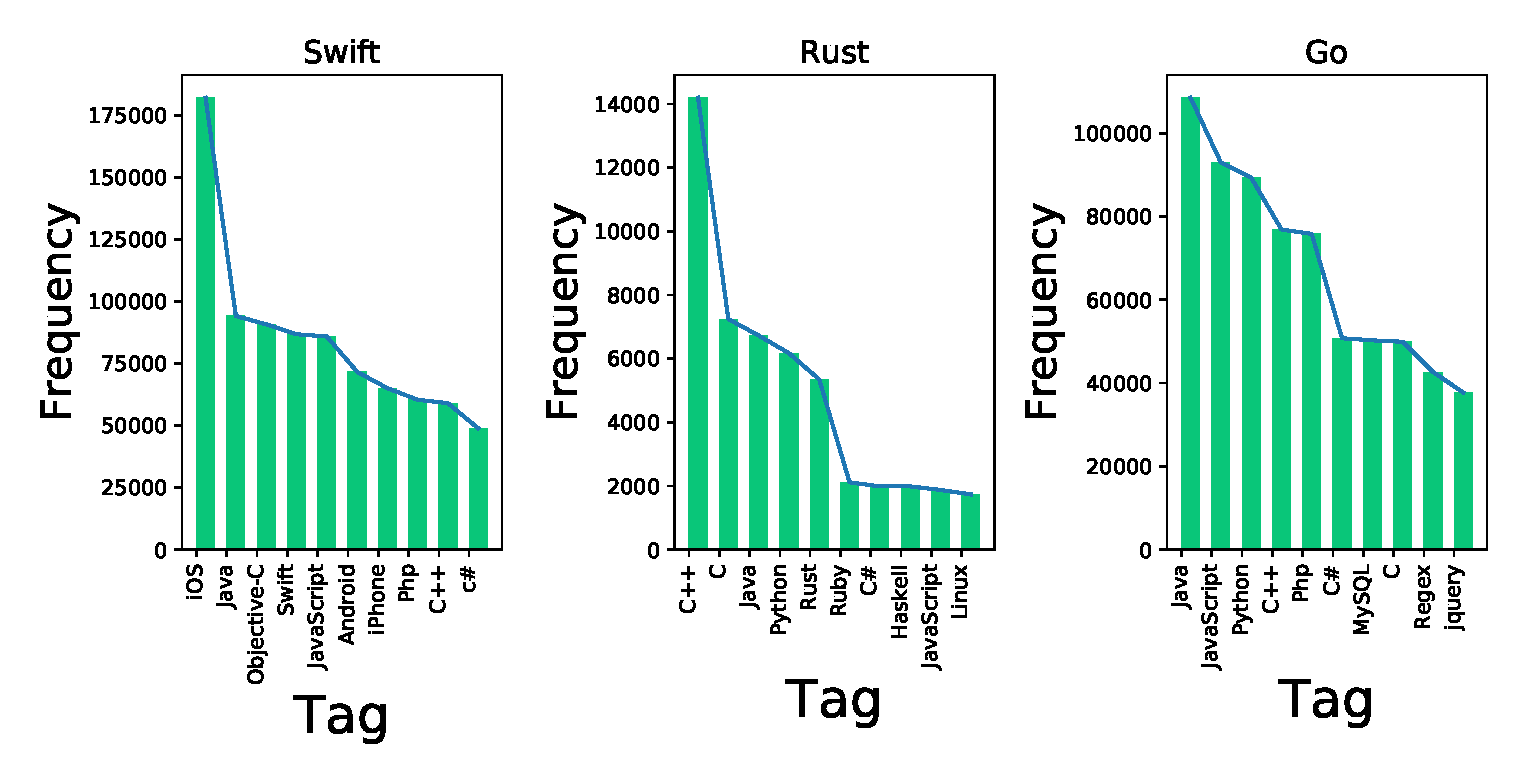
\includegraphics[scale=0.35]{figures/Tagfrequency.eps}
\caption{Most frequent 10 tags answered by expert developers of new languages.}
\label{fig:dev skills}
\end{figure}

Rust experts mostly answered  C and C++ questions. C++ is the predecessor language of Rust. Hence, we can say developers expert in Rust are also expert in C and C++. From that, we can infer that Rust is receiving contributions from the C and C++ community base in Stack Overflow. Developers expert in Swift have mostly answered the Java and Objective-C questions where Objective-C is considered the predecessor of Swift language. Therefore, it is evident that the new languages can get crucial support in their \emph{evolving state} if it has a predecessor language.

\boxtext{\textbf{Finding 9:} New languages are benefited from the community base of the predecessor language.}

